% Template per generare 

\documentclass[a4paper,11pt]{article}
\usepackage{lmodern}
\renewcommand*\familydefault{\sfdefault}
\usepackage{sfmath}
\usepackage[utf8]{inputenc}
\usepackage[T1]{fontenc}
\usepackage[italian]{babel}
\usepackage{indentfirst}
\usepackage{graphicx}
\usepackage{tikz}
\usepackage{listings}
\newcommand*\circled[1]{\tikz[baseline=(char.base)]{
		\node[shape=circle,draw,inner sep=2pt] (char) {#1};}}
\usepackage{enumitem}
% \usepackage[group-separator={\,}]{siunitx}
\usepackage[left=2cm, right=2cm, bottom=3cm]{geometry}
\frenchspacing

\newcommand{\num}[1]{#1}

% Macro varie...
\newcommand{\file}[1]{\texttt{#1}}
\renewcommand{\arraystretch}{1.3}
\newcommand{\esempioA}[2]{
\noindent\begin{minipage}{\textwidth}
\begin{tabular}{|p{7cm}|p{9cm}|}
	\hline
      \textbf{\file{input (da stdin)}} & \textbf{\file{output (su stdout)}}\\
	\hline
	\tt \small #1 &
	\tt \small #2 \\
	\hline
\end{tabular}
\end{minipage}
}
\newcommand{\esempioB}[2]{
\noindent\begin{minipage}{\textwidth}
\begin{tabular}{|p{9cm}|p{7cm}|}
	\hline
      \textbf{\file{input (da stdin)}} & \textbf{\file{output (su stdout)}}\\
	\hline
	\tt \small #1 &
	\tt \small #2 \\
	\hline
\end{tabular}
\end{minipage}
}

% Dati del task
\newcommand{\gara}{Esame Algoritmi 2019-09-04}
\newcommand{\nome}{Evaporazione dei nodi di livello dispari da un albero ordinato}
\newcommand{\nomebreve}{tree\_split\_out}

\begin{document}
% Intestazione
\noindent{\Large \gara}
\vspace{0.5cm}

\noindent{\Huge \textbf \nome~(\texttt{\nomebreve})}

% Descrizione del task
\section*{Descrizione del problema}

Un \emph{albero ordinato} consta di un \emph{nodo radice} e di una sequenza finita (eventualmente vuota) di \emph{figli} della radice, che sono a loro volta alberi ordinati. La figura offre tre rappresentazioni dello stesso albero, nella prima su ogni nodo viene riportato il numero dei suoi figli, nella seconda dei discendenti (incluso il nodo stesso), nella terza viene indicato il livello di ciascun nodo, ossia la sua distanza dalla radice. Per convenzione, la radice viene disegnata in cima (cio\`e al contrario rispetto agli alberi veri).

\begin{figure}[h!]
  \centering
    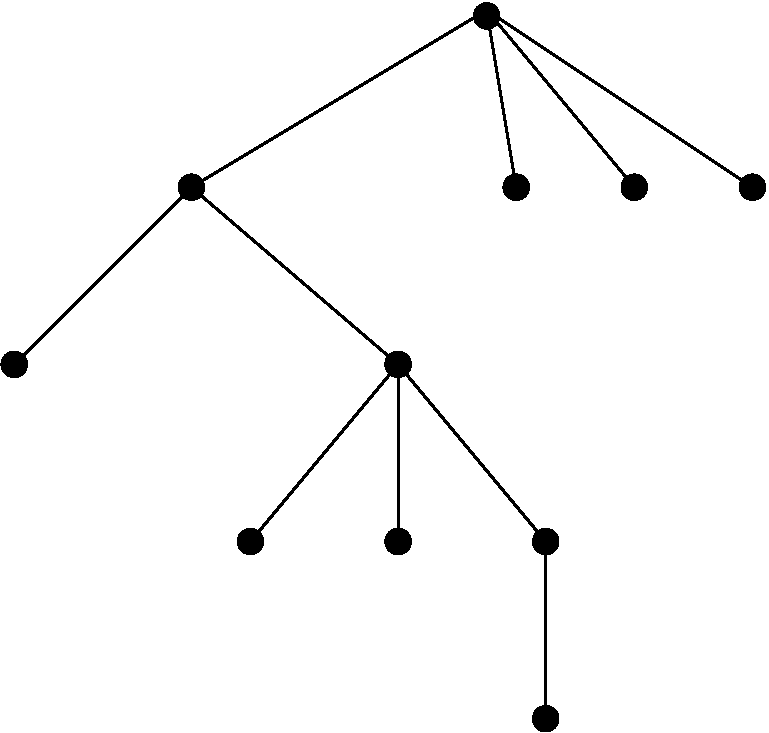
\includegraphics[scale=0.24]{figs/fig1.pdf}
      \quad \quad \quad
    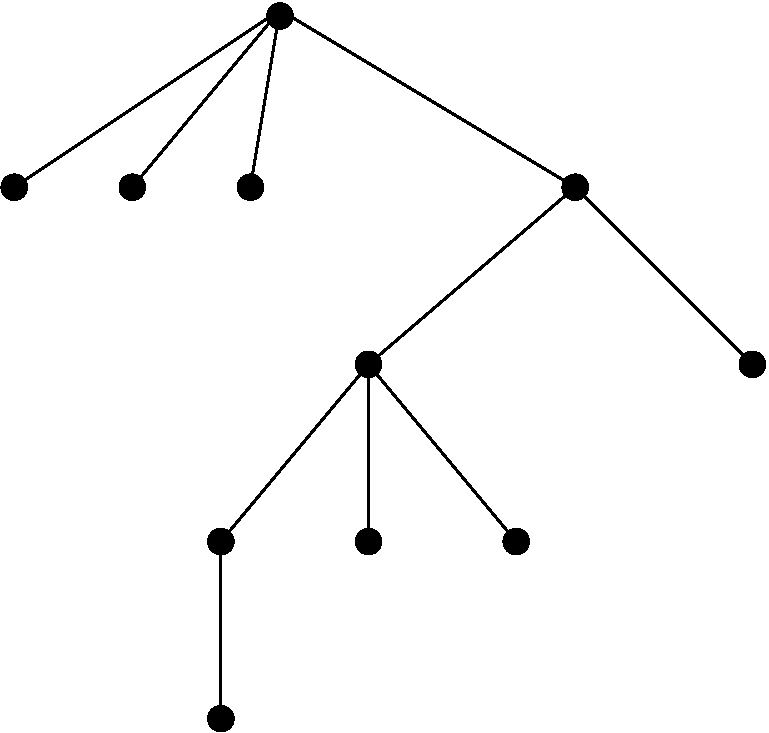
\includegraphics[scale=0.24]{figs/fig2.pdf}
      \quad \quad \quad
    \includegraphics[scale=0.24]{figs/fig3.pdf}
      \quad \quad \quad
    \includegraphics[scale=0.24]{figs/fig4.pdf}
    \caption{Un albero dove ogni nodo dichiara: il numero dei propri figli (a sinistra), il numero dei propri discendenti (in centro), il proprio livello (a destra). Infine l'albero ottenuto per evaporazione dei nodi di livello dispari.}
\end{figure}

\medskip

    {\bf Evaporazione di un nodo:}
    Al nodo radice non è concesso di evaporare a meno che esso stesso sia una foglia (ossia non abbia figli).
    Quando un nodo foglia evapora esso semplicemente sparisce.
    In tutti gli altri casi il nodo sparisce e la sequenza ordinata dei suoi figli prende il suo posto entro la sequenza ordinata della lista dei figli del padre.\\ 

\medskip

\noindent
Proponiamo tre possibili modi di codificare un albero con una sequenza di numeri naturali. Il primissimo numero della sequenza ($1$ oppure~$2$ o~$3$) specifica la codifica scelta.\\

\noindent
{\bf Codifica~1:}
Nella prima codifica, il primo numero è $1$, ed è seguito da tanti numeri naturali quanti sono i nodi dell'albero. In pratica ogni nodo dichiara a turno il numero dei propri figli, partendo dalla radice e nell'ordine della visita in profondità che rispetta tutti gli ordinamenti tra fratelli.
Possiamo definire tale sequenza in modo ricorsivo, impiegando la stessa decomposizione ricorsiva utilizzata sopra per definire gli alberi:
l'albero viene descritto dicendo quanti figli ha la radice (in questo caso, quattro) e poi descrivendo uno a uno, nell'ordine da sinistra a destra, i quattro sottoalberi. In questo modo, ad esempio, l'albero in figura sarebbe identificato dalla seguente sequenza:
\[
1\,\,\,4\,\,\,2\,\,\,0\,\,\,3\,\,\,0\,\,\,0\,\,\,1\,\,\,0\,\,\,0\,\,\,0\,\,\,0
\]      
Infatti, l'albero ha quattro figli sotto la radice, per cui il primo numero dopo lo specificatore di formato ($1$) \`e $4$. A questo $4$ segue poi subito la sequenza $2\,\,\,0\,\,\,3\,\,\,0\,\,\,0\,\,\,1\,\,\,0$, che \`e la descrizione del primo figlio, mentre gli ultimi tre figli sono ciascuno descritti da $0$ (dato che non hanno figli).\\

\noindent
{\bf Codifica~2:}
Comincia con un $2$,
di nuovo seguito da una sequenza di tanti numeri naturali quanti sono i nodi dell'albero.
I nodi parlano nello stesso ordine visto sopra ma questa volta ogni nodo dichiara il numero dei propri discendenti (incluso sè stesso).
Equivalentemente, l'albero viene descritto dicendo quanti discendenti ha la radice (in questo caso 11) e poi descrivendo uno a uno, nell'ordine da sinistra a destra, i quattro sottoalberi. In questo modo, ad esempio, l'albero in figura sarebbe identificato dalla seguente sequenza:
\[
2\,\,\,11\,\,\,7\,\,\,1\,\,\,5\,\,\,1\,\,\,1\,\,\,2\,\,\,1\,\,\,1\,\,\,1\,\,\,1
\]	

Infatti, l'albero ha 11 nodi in tutto, ossia 11 sono i discendenti della radice (ogni nodo si considera discendente di se stesso), per cui il primo numero dopo lo specificatore di formato ($1$) \`e $11$. A questo $11$ segue poi subito la sequenza $7\,\,\,1\,\,\,5\,\,\,1\,\,\,1\,\,\,2\,\,\,1$, che \`e la descrizione del primo sottoalbero, mentre gli ultimi tre sottoalberi sono ciascuno descritti da $1$ (dato che non hanno alcun figlio).\\

\noindent
{\bf Codifica~3:}
Comincia con un $3$,
ma quì la sequenza a seguire è lunga il doppio in quanto ogni nodo parla due volte:
sia in apertura che in chiusura del sottoalbero di cui egli è radice.
In entrambe le occasioni, il nodo dice il proprio livello entro l'albero, ossia il numero di archi nell'unico cammino che lo collega alla radice.
Apertura e chiusura coincidono col primo e l'ultimo passaggo per il nodo da parte della visita in profondità che rispetta tutti gli ordinamenti tra fratelli.
Pertanto, l'ordine in cui ogni sottoalbero viene aperto ed il nodo parla per la prima volta è lo stesso che per le Codifiche~1 e~2. 
La terza codifica dell'albero in figura è la seguente:
\[
3\,\,\,0\,\,\,1\,\,\,2\,\,\,2\,\,\,2\,\,\,3\,\,\,3\,\,\,3\,\,\,3\,\,\,3\,\,\,4\,\,\,4\,\,\,3\,\,\,2\,\,\,1\,\,\,1\,\,\,1\,\,\,1\,\,\,1\,\,\,1\,\,\,1\,\,\,0
\]	



% Input
\section*{Dati di input}

L'input deve avvenire da stdin, da dove il vostro programma legge una sola riga contenente la codifica di un albero offerta secondo uno dei tre formati definiti sopra.

% Output
\section*{Dati di output}

L'output deve avvenire su stdout, dove il vostro programma deve restituire una sola riga:
la codifica, nello stesso formato dell'input, dell'albero ottenuto per evaporazione di tutti i nodi di livello dispari entro l'albero assegnato.

% Esempi
\section*{Esempio di input/output}

\esempioB{
1 4 2 0 3 0 0 1 0 0 0 0
}{
1 2 0 1 0  
}

\medskip
\bigskip
\esempioB{
2 11 7 1 5 1 1 2 1 1 1 1
}{
2 4 1 2 1
}

\medskip
\bigskip
\esempioB{
3 0 1 2 2 2 3 3 3 3 3 4 4 3 2 1 1 1 1 1 1 1 0
}{
3 0 1 1 1 2 2 1 0
}

%Assunzioni
%\section*{Assunzioni}
%\begin{itemize}[nolistsep, noitemsep]
%\item dove $n$ \`e il numero di nodi dell'albero,
%      vale sempre che $1 \le n \le 300\,000 $;
%\item tempo limite: un secondo.
%\end{itemize}

% Subtasks
\section*{Subtask}

\begin{itemize}
\item \textbf{Subtask 1 [0 punti]:} i casi di esempio forniti alla pagina del problema, essi includono i tre casi sopra.
\item \textbf{Subtask 2 [10 punti]:} Codifica~3, $N \le 10$.
\item \textbf{Subtask 3 [10 punti]:} Codifica~3, $N \le 1000$.
\item \textbf{Subtask 4 [10 punti]:} Codifica~3, $N \le 300\,000$.
\item \textbf{Subtask 5 [11 punti]:} Codifica~2, $N \le 10$.
\item \textbf{Subtask 6 [11 punti]:} Codifica~2, $N \le 1000$.
\item \textbf{Subtask 7 [12 punti]:} Codifica~2, $N \le 300\,000$.
\item \textbf{Subtask 8 [12 punti]:} Codifica~1, $N \le 10$.
\item \textbf{Subtask 9 [12 punti]:} Codifica~1, $N \le 1000$.
\item \textbf{Subtask 10 [12 punti]:} Codifica~1, $N \le 300\,000$.
\end{itemize}

I subtask in Codifica~3 dovrebbero risultare più facili, per questo li abbiamo collocati per primi.

\end{document}
